% !TEX program = pdflatex
% Powder-Excavator design brainstorming and prior-art review.
%
% Build:
%   cd docs/manuscript
%   pdflatex main
%   bibtex   main
%   pdflatex main
%   pdflatex main
%
% Or use the Makefile in this directory: ``make``.

\documentclass[11pt,a4paper]{article}

\usepackage[margin=1in]{geometry}
\usepackage[utf8]{inputenc}
\usepackage[T1]{fontenc}
\usepackage{lmodern}
\usepackage{microtype}
\usepackage{textcomp}
\usepackage[hyphens]{url}
\usepackage{xcolor}
\usepackage{hyperref}
\hypersetup{
  colorlinks=true,
  linkcolor=blue!50!black,
  citecolor=blue!50!black,
  urlcolor=blue!50!black,
  pdftitle={Powder-Excavator: design brainstorming and prior-art notes},
  pdfauthor={vertical-cloud-lab},
}
\usepackage{enumitem}
\usepackage{graphicx}
\usepackage{booktabs}
\usepackage{tabularx}
\usepackage{longtable}
\usepackage{caption}
\usepackage{siunitx}

\sisetup{
  range-units = single,
  per-mode    = symbol,
}

\title{Powder-Excavator: design brainstorming and prior-art notes}
\author{vertical-cloud-lab}
\date{April 2026}

\begin{document}
\maketitle

\begin{abstract}
\noindent
This document captures a literature-aware brainstorm for the gantry-mounted
``powder excavator'' sketched in \texttt{powder-excavator-sketch.jpg} and
recreated as the labelled subpanels under \texttt{docs/figures/}. It is
structured roughly like the introduction to a \emph{Digital Discovery}
manuscript on a new powder-handling tool: where does this device sit in the
landscape of automated powder dispensing, what gap is it trying to fill, and
what would we need to measure to defend that claim. The current revision
adopts the corrected \emph{longitudinal-pivot, sideways-tilt} geometry
identified by the Edison Scientific design-review tasks~\cite{edisonscientific},
and adds a cam-slot / pin-defined-path actuation variant (Sec.~\ref{sec:pinslot})
based on a follow-on hand sketch.
\end{abstract}

\paragraph{Provenance.}
This brainstorm was prompted by feedback on PR~\#2 to ``send the idea to
Edison for a high-effort literature search'' and to consider the discussion
at the Accelerated Discovery
thread~\cite{accdiscthread}. The Edison Scientific service was wired in via
\texttt{edison\_client} for a follow-up session: a high-effort PaperQA3
literature search and two high-effort design-review tasks were
run~\cite{edisonscientific}, and their verbatim responses are archived under
\texttt{docs/edison/}. Peer-reviewed citations marked
\cite{tom2024selfdrivinglaboratoriesfor,yang2007meteringanddispensing,bahr2018collaborativeevaluationof,bahr2020recentadvancesin,jiang2023autonomousbiomimeticsolid,szymanski2023anautonomouslaboratory,szymanski2024automatingthesynthesis,fei2024alabosapythonbased,lunt2023modularmultirobotintegration,lunt2024aroboticworkflow,carruthers2025amobilerobotic,alsenz2011powderpickinganinexpensive,hernandezdelvalle2024pelletdispensomixerand,doloi2025democratizingselfdrivinglabs,moravkar2020traditionalandadvanced,freeman2017characterisingpowderflow,ghoroi2013multifacetedcharacterizationof,mccalla2023semiautomatedexperimentsto}
are taken directly from the Edison literature task and are listed in the
\hyperref[sec:references]{References} section.

\paragraph{Geometry note (post-review).}
The mechanism described in Sec.~\ref{sec:fits} and Sec.~\ref{sec:variations}
has been updated to the \textbf{longitudinal-pivot, sideways-tilt,
smooth-cam-ramp} geometry adopted after the Edison design-review tasks
identified two design-blocking issues with the earlier ``ferris-wheel
gondola'' (transverse pivot, end-over-end tilt, sawtooth and hooked-lip)
revision: a kinematic impossibility in the push-to-tilt mechanism and a
trapped-volume / bridging problem for cohesive powders. Section~\ref{sec:pinslot}
adds a \emph{pin-defined-path} actuation variant in which a peg on a stem
descending from the gantry rides in a routed slot in a fixed external board;
this captures the cam-ramp idea in a fully constrained ``peg in slot'' form
that removes the approach/contact ambiguity of a free cam follower.

% --------------------------------------------------------------------------
\section{Why powder handling is the pinch point in self-driving labs}
\label{sec:why}

Self-driving laboratories (SDLs) for chemistry and materials science have
matured rapidly over the past five years, with closed-loop platforms now
routinely combining robotic execution, automated characterization, and
Bayesian or generative experiment design~\cite{tom2024selfdrivinglaboratoriesfor,szymanski2023anautonomouslaboratory,fei2024alabosapythonbased,mccalla2023semiautomatedexperimentsto}.
Across nearly every published SDL, \textbf{solids handling --- and powder
dispensing in particular --- is repeatedly called out as the dominant
bottleneck}: it is the step most likely to be left to a human, the one most
sensitive to material properties (cohesion, hygroscopicity, triboelectric
charging), and the one that most often limits end-to-end
autonomy~\cite{tom2024selfdrivinglaboratoriesfor,yang2007meteringanddispensing,carruthers2025amobilerobotic,jiang2023autonomousbiomimeticsolid}.
Tom et al.'s 2024 \emph{Chemical Reviews} survey of SDLs makes the point
bluntly: solid-dispensing hardware ``remains rare and costly relative to
liquid handling, and many labs simply avoid direct powder
manipulation'' wherever pre-dissolved stocks will
do~\cite{tom2024selfdrivinglaboratoriesfor}.

Compared with liquid handling, powder dispensing is hard for three coupled
reasons:

\begin{enumerate}[leftmargin=*]
  \item \textbf{No universal flow regime.} Free-flowing crystalline powders,
    fluffy nanopowders, sticky organics, and hygroscopic salts each demand
    different feeders, hoppers, and tip
    geometries~\cite{yang2007meteringanddispensing,bahr2018collaborativeevaluationof,carruthers2025amobilerobotic}.
  \item \textbf{Dose accuracy scales poorly down.} Sub-milligram gravimetric
    dosing needs a draft-shielded balance, vibration isolation, and feedback
    control; the 17{,}797-dispense ETC benchmark across four commercial
    platforms found that \SI{2}{\milli\gram} targets exhibited
    \SIrange{190}{680}{\percent} higher \%RSD than \SI{50}{\milli\gram}
    targets, and that across the full dataset the percent error spanned
    \SI{-10}{\percent} to \SI{+3245}{\percent} (\SI{95.3}{\percent} of
    dispenses fell between \SI{-25}{\percent} and
    \SI{+100}{\percent})~\cite{bahr2018collaborativeevaluationof,bahr2020recentadvancesin}.
  \item \textbf{Cross-contamination is expensive.} Reservoirs and
    end-effectors must either be disposable, easily cleaned, or dedicated
    per material, which blows up the part count of a multi-reagent
    platform~\cite{tom2024selfdrivinglaboratoriesfor,carruthers2025amobilerobotic}.
\end{enumerate}

% --------------------------------------------------------------------------
\section{Prior art (representative, not exhaustive)}
\label{sec:priorart}

Table~\ref{tab:priorart} summarises the device classes that any new
powder-handling tool has to position itself against. The rows are not
intended as a complete vendor list; they are the classes of mechanism that
recur across the SDL literature
\cite{tom2024selfdrivinglaboratoriesfor,yang2007meteringanddispensing,bahr2018collaborativeevaluationof,bahr2020recentadvancesin,jiang2023autonomousbiomimeticsolid,szymanski2023anautonomouslaboratory,fei2024alabosapythonbased,lunt2023modularmultirobotintegration,lunt2024aroboticworkflow,carruthers2025amobilerobotic,alsenz2011powderpickinganinexpensive}.

\begin{small}
\begin{longtable}{@{}p{0.21\linewidth}p{0.36\linewidth}p{0.36\linewidth}@{}}
\caption{Prior-art device classes for automated powder handling. Quantitative
claims in the ``Strengths'' and ``Limits'' columns are taken from the cited
sources.}
\label{tab:priorart}\\
\toprule
\textbf{Class} & \textbf{Strengths} & \textbf{Limits relevant to us} \\
\midrule
\endfirsthead
\multicolumn{3}{c}{\tablename\ \thetable{} -- continued from previous page}\\
\toprule
\textbf{Class} & \textbf{Strengths} & \textbf{Limits relevant to us} \\
\midrule
\endhead
\midrule
\multicolumn{3}{r}{\emph{continued on next page}}\\
\endfoot
\bottomrule
\endlastfoot
Gravimetric vibratory-head dispensers (Quantos QX1/QX5, Chemspeed SWING /
Powdernium / FLEX GDU-Pfd, Unchained Labs Freeslate/Junior) &
High precision on dense free-flowing powders; closed-loop weight feedback;
integrated workflow software; ETC benchmark established Quantos as the best
overall \% error / \%RSD / time balance and Chemspeed SWING as the fastest
(\SIrange{13}{65}{\second})~\cite{bahr2018collaborativeevaluationof,bahr2020recentadvancesin} &
Per-reagent consumable cartridges/heads; abrasive solids damage Quantos
heads; hygroscopic powders clog them; Chemspeed SWING and one Unchained
system \emph{failed outright} on fumed silica in the ETC
benchmark~\cite{bahr2018collaborativeevaluationof,carruthers2025amobilerobotic} \\
\addlinespace
Auger / screw feeders on robot arms (Berlinguette \& MacLeod ``Ada''
thin-film SDL; Aspuru-Guzik group platforms; Chemspeed FLEX GDU-Pfd
hopper/auger module) &
Robust to mildly cohesive powders; metered dosing; \SI{\pm10}{\percent}
tolerance setting on GDU-Pfd~\cite{bahr2020recentadvancesin} &
Mechanical complexity; cleaning between materials non-trivial; the Lunt
modular-workflow paper notes ``grinding, mixing and recovering solids
remains an unsolved challenge in commercial
automation''~\cite{lunt2023modularmultirobotintegration,lunt2024aroboticworkflow} \\
\addlinespace
Spatula-mimicking dual-arm robots (Cooper group's
PowderBot~\cite{jiang2023autonomousbiomimeticsolid}) &
Versatile across material classes; \(\sim\)\SI{0.07}{\percent} error at
\SI{200}{\milli\gram} for non-challenging solids; comparable failure rate
to commercial systems (\SI{23.1}{\percent} vs.\ \SI{26.9}{\percent} vs.\
\SI{26.5}{\percent}) at lower hardware
cost~\cite{jiang2023autonomousbiomimeticsolid} &
Slow throughput due to manipulator motions and corrective restarts;
struggles with compressible powders (CaCO\textsubscript{3}) and highly
hygroscopic materials~\cite{jiang2023autonomousbiomimeticsolid} \\
\addlinespace
Slurry-conversion workflows (Ceder group A-Lab: Quantos doses precursors
into vials, ball-milled with ethanol into pumpable
slurry)~\cite{szymanski2023anautonomouslaboratory,szymanski2024automatingthesynthesis,fei2024alabosapythonbased} &
Sidesteps last-mile dry-transfer issues; well-characterised end-to-end
workflow; 36 novel compounds in 17 days &
Adds ethanol handling, drying, and a dedicated \texttt{RecoverPowder}
regrinding task downstream; upstream powder loading is still
manual~\cite{szymanski2024automatingthesynthesis} \\
\addlinespace
Capsule / cartridge ``drop a pre-weighed slug'' &
Eliminates real-time dosing error &
Needs upstream weighing; Quantos cartridge ecosystem in particular
criticised for high cost, single-vendor procurement, RFID-locked reuse,
and clogging on hygroscopic
powders~\cite{carruthers2025amobilerobotic} \\
\addlinespace
Acoustic / ultrasonic non-contact transfer (Echo-style platforms; ultrasonic
capillaries, \SIrange{14}{16}{\micro\gram} through \SI{0.2}{\milli\meter}
nozzles)~\cite{yang2007meteringanddispensing} &
Non-contact, no cross-contamination, very high throughput &
Limited to specific particle sizes / suspensions; mostly demonstrated in
solid-freeforming / additive-manufacturing contexts, not chemistry SDLs \\
\addlinespace
Vacuum / electrostatic pickup (DryPette, Electronic Spatula, automated
electrostatic pipettes)~\cite{yang2007meteringanddispensing,alsenz2011powderpickinganinexpensive} &
Gentle on the powder; good for fragile crystals; \SI{0.3}{\milli\gram}-class
doses possible &
Hard to release a clean dose; \emph{exquisitely} sensitive to humidity,
charge decay, and powder conductivity~\cite{yang2007meteringanddispensing} \\
\addlinespace
Positive-displacement ``PowderPicking'' (standard Gilson MICROMAN pipettes
with disposable capillary-piston tips,
Alsenz)~\cite{alsenz2011powderpickinganinexpensive,cook2021guideto} &
Cheap; \SIrange{0.6}{25}{\milli\gram} range; mean CV \(\sim\)\SI{6}{\percent}
across 10 powders; disposable tips eliminate carryover &
Manual / medium throughput; depends on complete homogeneous filling of the
probe cylinder; tip clogging with adhesive
powders~\cite{alsenz2011powderpickinganinexpensive} \\
\addlinespace
Bulk ``scoop and dump'' mechanical scoops (\textbf{this project}; closest
commercial analogue: MTI PF-A glass dispenser referenced in the community
thread)~\cite{mtipfaglassdispenser} &
Cheap, mechanically simple, no actuators on the end-effector, easy to clean;
the present design has \emph{no consumable} at all &
Not a precision dosing tool; dose CV likely \SIrange{5}{20}{\percent}
depending on whether a strike-off bar is used; not for sub-mg work \\
\end{longtable}
\end{small}

Two recent overviews are particularly relevant for situating a new device
in this landscape: Tom et al.'s 2024 \emph{Chemical Reviews}
survey~\cite{tom2024selfdrivinglaboratoriesfor} and Lunt et al.'s
solid-state-workflow papers~\cite{lunt2023modularmultirobotintegration,lunt2024aroboticworkflow}.
Both flag \emph{bulk powder transfer from stock containers into a precision
dispenser} as a step that is still almost universally manual. On the
frugal-hardware side, recent open-hardware platforms have demonstrated cost
reductions of up to \SI{94}{\percent} relative to commercial analogues for
adjacent dispensing problems (pellet dispensers, 3D-printed
autosamplers)~\cite{hernandezdelvalle2024pelletdispensomixerand,doloi2025democratizingselfdrivinglabs},
albeit for liquid or pellet handling rather than fine inorganic powders.

\subsection{Community prior art from the Accelerated Discovery thread}
\label{sec:thread}

The Accelerated Discovery thread ``Accurate powder dispensing for chemistry
and materials science applications''~\cite{accdiscthread} is a useful,
opinionated cross-section of what practitioners have actually tried. The
points most relevant to our design:

\begin{itemize}[leftmargin=*]
  \item \textbf{Framing (sgbaird, post 1).} Accurate powder dispensing is
    ``around an order of magnitude more complex and more expensive than
    liquid handling.''  This matches the SDL
    surveys~\cite{tom2024selfdrivinglaboratoriesfor} and is the gap we are
    trying to chip away at on the cheap, mechanical end of the design space.
  \item \textbf{3D-printed calibrated spatulas (post 2, after Cook
    et al.~\cite{cook2021guideto}).} Sets of spatulas with known volumes
    give a calibration curve from volume to mass; decent accuracy in
    isolation, but degraded by static in gloveboxes and by lighter powders.
    Two takeaways for us: (i) \textbf{a strike-off bar is essentially
    required} (``just manually tapped the spatula until each scoop is level
    \dots\ it doesn't seem too difficult to physically level it by passing
    something against the top of the scoop'') --- directly endorses the
    strike-off bar variant in Sec.~\ref{sec:variations}; (ii) per-material
    calibration is realistic if the trough is geometrically well-defined.
  \item \textbf{Positive-displacement-pipette method (post 3,
    Alsenz~\cite{alsenz2011powderpickinganinexpensive}).} Packs a pipette
    tip into the powder; spans \SIrange{0.6}{20}{\milli\gram} with
    \(\sim\)\SI{10}{\percent} CV across tip sizes. The
    \SI{10}{\percent} CV is a \textbf{useful baseline target} for our scoop
    on cohesive powders.
  \item \textbf{Auger / screw-feed builds (loppe35, post 4).} Cheap (jewelry-
    scale load cell \(\approx\) USD 25, stepper + control board) but ``leaky
    when dispensing vertically'' and needs hopper flow aids. Reinforces
    keeping the excavator's bucket \emph{un-augered} in the baseline design;
    the auger is positioned in Sec.~\ref{sec:variations} as an optional
    add-on, not the core mechanism.
  \item \textbf{The ``pick it back up'' problem (muon, posts 5/7/14).}
    Dispensing is only half the workflow; recovering powder \emph{after}
    an operation (ball-milling, acoustic mixing, weighing) is at least as
    hard, and a vacuum/pipette approach is awkward when the milled powder
    is fine and multi-precursor cross-contamination matters.
  \item \textbf{Autotrickler v4 + A\&D FX-120i (sgbaird, post 6).}
    \SI{\pm1}{\milli\gram}, fast-response scale, BLE-controllable from a
    Pico W; community-validated reference for the ``scale + metered feed''
    downstream of a bulk-transfer device. Suggests a concrete integration
    target: excavator $\rightarrow$ tared Autotrickler-style
    trickler/scale.
  \item \textbf{PowderBot (Cooper group)~\cite{jiang2023autonomousbiomimeticsolid}
    and A-Lab (Ceder
    group)~\cite{szymanski2023anautonomouslaboratory,fei2024alabosapythonbased}.}
    Two published end-to-end SDLs that \emph{did} solve solids handling, but
    with workflow-specific workarounds (typically involving milling).
  \item \textbf{Manual MTI PF-A glass dispenser (sgbaird, post~24 --- the
    specific post linked in the review feedback)~\cite{mtipfaglassdispenser}.}
    A \SI{250}{\milli\litre} hand dispenser whose geometry is reminiscent
    of Owen Melville's earlier scoop. The closest existing artifact to our
    bucket and effectively a manual ancestor of the excavator's scoop motion.
\end{itemize}

% --------------------------------------------------------------------------
\section{Where the powder-excavator fits}
\label{sec:fits}

The proposed mini excavator is \textbf{not} competing with Quantos-class
precision dispensers. It is aimed at the \textbf{upstream, bulk-transfer
step}: moving a relatively coarse aliquot of powder from a stock bed (e.g.\
a tray, jar, or hopper) to a downstream station --- which might itself be
a precision dispenser, a sieve, a press, a crucible, a dissolution vial,
or simply a weigh boat for a human-in-the-loop workflow. In that niche, the
design choices shown in Fig.~\ref{fig:panels} (post-review) make sense:

\begin{itemize}[leftmargin=*]
  \item \textbf{Half-cylinder ladle suspended on a longitudinal pivot pin.}
    The pin runs along the trough's long axis $L$, through the two short
    end caps, with the two arms gripping those end caps. The trough rolls
    \emph{sideways} about the pin to pour, dispensing over the
    \emph{full long edge} rather than through a narrow end-cap point. This
    eliminates the trapped-volume / arching failure mode that an end-over-
    end tilt of a half-cylinder would have for cohesive powders (Edison v2
    \S3, archived in \texttt{docs/edison/}).
  \item \textbf{Pure mechanical actuation via a fixed smooth inclined cam
    ramp.} Removes the servo and its wiring/maintenance burden; the deposit
    angle is set by how far up the cam the trough's chamfered bumper has
    ridden (i.e.\ by gantry $X$ position), not by a torque setpoint. A
    smooth ramp --- rather than a sawtooth tooth --- is required because a
    fixed point engaging a fixed-radius hook on a horizontally-translating
    pivot is geometrically impossible (Edison v2 \S1).
    Sec.~\ref{sec:pinslot} below describes a stricter ``peg in routed slot''
    refinement of this idea.
  \item \textbf{Mandatory bed-edge strike-off bar.} Promoted from
    ``optional variation'' to a baseline-required part: without a
    level-defining strike-off, dose CV will sit in the
    \SIrange{15}{30}{\percent} range across powder classes, which would
    put the device below the \(\approx\) \SI{10}{\percent} CV baseline
    achievable with Alsenz's positive-displacement-pipette
    method~\cite{alsenz2011powderpickinganinexpensive} and below the
    Cooper PowderBot's \SI{0.07}{\percent} at
    \SI{200}{\milli\gram}~\cite{jiang2023autonomousbiomimeticsolid}.
  \item \textbf{Open top with no lid.} Trades some retention loss for
    radically simpler cleaning --- which, per
    \cite{tom2024selfdrivinglaboratoriesfor,carruthers2025amobilerobotic},
    is the single biggest hidden cost in multi-material SDLs.
  \item \textbf{Optional grounded conductive lining.} Because the pivot
    pin is a metal dowel, it can double as the ground path for an
    inexpensive copper-tape lining of the trough interior. This is the
    prototype-friendly equivalent of using ESD-safe filament and
    dramatically reduces triboelectric charging on fine inorganics
    (Edison v1 \S2).
\end{itemize}

A reasonable framing for a write-up: \emph{``A purely mechanical,
gantry-mounted ladle for bulk powder transfer in self-driving materials
labs, designed to bridge stock containers and precision dispensers without
adding servo count or cleaning burden, and to take over the upstream-loading
and post-process recovery roles flagged as unsolved by Lunt
et al.''}~\cite{lunt2023modularmultirobotintegration,lunt2024aroboticworkflow}.

The design intentionally makes \textbf{no claim} of being a precision
dispenser, and tempers the ``bidirectional dispense + recover'' claim made
in earlier framing: a half-cylinder cannot scoop cleanly out of a flat bed
without leaving a trail of retained powder, so recovery is a meaningful but
lossy operation rather than a complete one (Edison v2 \S7).

% --------------------------------------------------------------------------
\section{Pin-defined-path actuation: a routed-slot refinement}
\label{sec:pinslot}

A hand-sketch (\texttt{PXL\_20260423\_231729467.jpg}) suggests an actuation
refinement that fully resolves the ``approach-and-contact'' ambiguity of
the smooth cam ramp described in Sec.~\ref{sec:fits}. Rather than a free
cam follower that approaches a fixed inclined surface and slides up it, the
trough is suspended from the gantry carriage by a short \emph{stem} that
carries a transverse \emph{peg} at its top end. This peg rides in a
\emph{routed slot} cut into a fixed external board mounted at fixed height
in the work area (Fig.~\ref{fig:pinslot}). The carriage--stem joint is a
pin pivot; the peg is captured in the slot for the entire stroke. Pure-$X$
gantry travel therefore drives a deterministic tilt-vs.-$X$ schedule given
by the slot's routed path: where the slot is straight and horizontal the
trough holds level (scoop, transport); where it deviates, the difference
between the carriage's straight-line path and the slot's routed path forces
the stem (and the trough rigidly attached to it) to rotate about the
carriage pivot.

This is mechanically the same idea as the cam paths used in coin-op
mechanisms, player pianos, and Geneva-style indexing devices, applied to
the gantry geometry of a self-driving lab. Compared with the smooth
inclined cam ramp of Sec.~\ref{sec:fits}, the pin-in-slot refinement has
several concrete advantages:

\begin{itemize}[leftmargin=*]
  \item \textbf{No engagement event.} The peg never has to ``find'' the
    cam; it is captive in the slot from the moment the trough is mounted.
    There is no lift-off direction in which the contact can lose registration.
  \item \textbf{Bidirectional and reversible.} The slot path constrains
    motion in both $+X$ and $-X$ directions, so the trough can be tipped,
    held, and \emph{returned to level} purely by gantry motion. The smooth
    cam ramp relies on gravity for the return.
  \item \textbf{Programmable schedule.} The slot is the program. Different
    routed slots --- straight-then-rising, multi-stage with a hold detent,
    a small ``knock'' wiggle to dislodge bridges (Edison v1 \S6) ---
    implement different dispensing schedules without any change to the
    trough or carriage. The strike-off bar sweep can be encoded as a small
    detent in the slot near the bed-edge $X$ coordinate.
  \item \textbf{Deterministic tilt at deposit.} Because the peg is captured
    on both sides of the slot wall, the deposit angle is set by slot
    geometry to the tolerance of the routing operation, not by friction at
    a sliding cam interface.
  \item \textbf{Simpler statics analysis.} The slot wall provides both the
    tilt-up reaction force and (on the return stroke) the tilt-down force.
    The smooth cam ramp only provides the former; the latter relies on
    gravity, which fails for very light troughs or when the trough is empty.
\end{itemize}

\paragraph{Caveats.} The slot must be cut to the same accuracy as the
finished tilt schedule requires; a cleanly milled slot in acrylic or
aluminium is straightforward, but FDM-printed slots will have layer-line
ripples that the peg will feel as a low-amplitude tilt jitter. The peg
should be a hardened dowel pin with a low-friction sleeve (PTFE or oil-
impregnated bronze) to minimise stick-slip, and the slot should be slightly
oversized in the direction perpendicular to the desired motion to allow
thermal play without binding. The board itself becomes a second
\emph{registered} fixture in the work area --- it must be mounted in a
known relationship to the gantry's $X$ axis, which is the same registration
problem the bed and the deposit station already face, and so does not
introduce a new class of failure.

% Place the four-panel layout figure environment up here so it floats
% sensibly relative to the references that point at it.
\begin{figure}[ht]
  \centering
  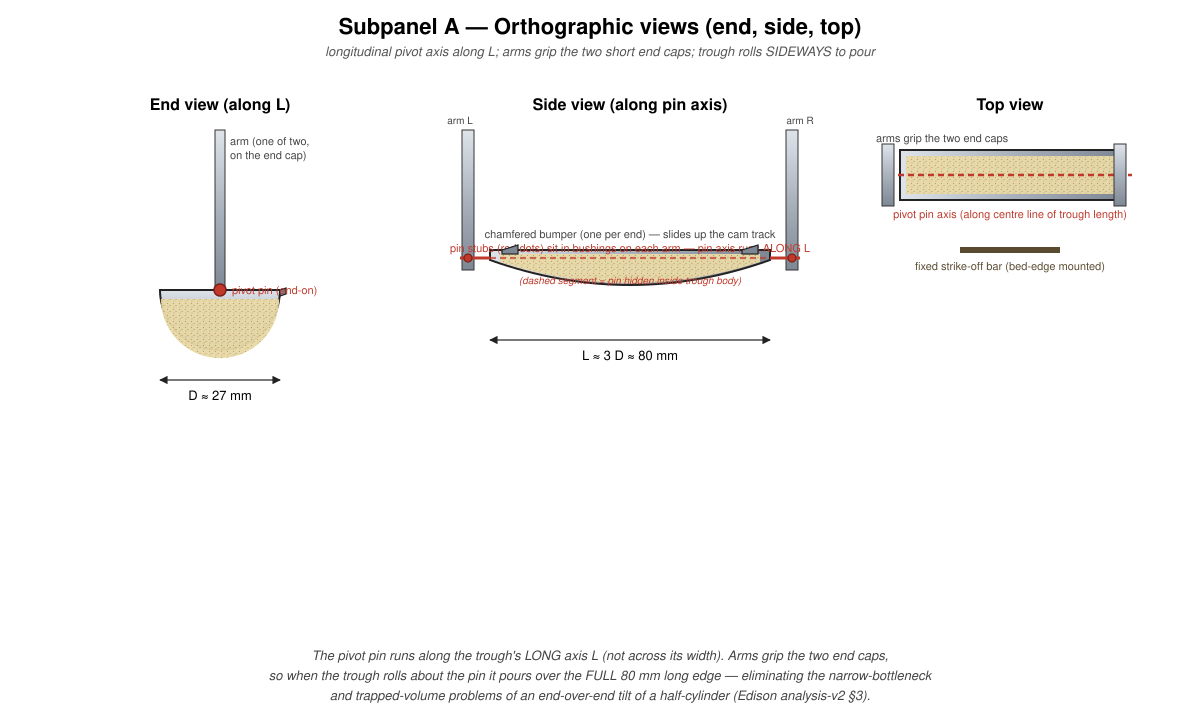
\includegraphics[width=0.95\linewidth]{../figures/panel-A-orthographic}
  \caption{Orthographic views of the half-cylinder trough with the
    longitudinal pivot pin, end-cap pivot bosses, and the chamfered bumper
    that engages the cam ramp. Generated by
    \texttt{scripts/generate\_figures.py}.}
  \label{fig:panels}
\end{figure}

\begin{figure}[ht]
  \centering
  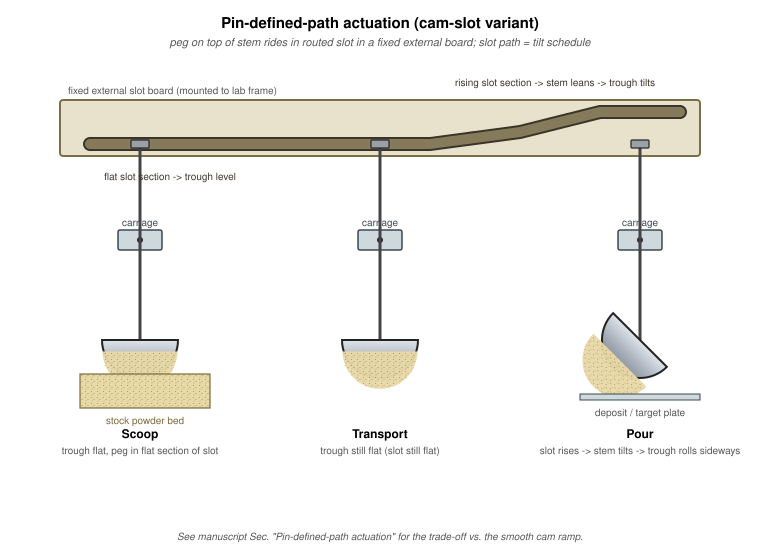
\includegraphics[width=0.85\linewidth]{../figures/panel-E-pin-slot}
  \caption{Pin-defined-path actuation variant (Sec.~\ref{sec:pinslot}). A
    vertical stem hangs from the gantry carriage on a pivot; a transverse
    peg at the top of the stem rides in a routed slot cut into a fixed
    external board. The slot's shape over $X$ is the program for the
    trough's tilt schedule. Generated by
    \texttt{scripts/generate\_figures.py}.}
  \label{fig:pinslot}
\end{figure}

% --------------------------------------------------------------------------
\section{Open questions and what we'd actually need to measure}
\label{sec:measure}

To defend the design in a manuscript-style argument we would need at
minimum:

\begin{itemize}[leftmargin=*]
  \item \textbf{Dose statistics across powder classes.} Mean and CV of
    delivered mass for at least three archetypal powders (e.g.\
    free-flowing crystalline like NaCl, cohesive metal-oxide nanopowder
    like TiO\textsubscript{2}, hygroscopic salt like LiCl) across at least
    30 scoops each. Following Cooper-group
    practice~\cite{jiang2023autonomousbiomimeticsolid}, this should also
    include the known ``hard'' cases --- fumed silica (which broke the
    Chemspeed SWING and one Unchained system in the ETC
    benchmark~\cite{bahr2018collaborativeevaluationof}) and CaCO\textsubscript{3}
    (which broke the PowderBot~\cite{jiang2023autonomousbiomimeticsolid}).
  \item \textbf{Standardised flowability descriptors per powder.} Report
    Carr's compressibility index (CI $\le$ \SI{10}{\percent} = excellent;
    \SIrange{21}{25}{\percent} = passable; $>$\SI{35}{\percent} = very poor)
    and the Hausner ratio (HR \numrange{1.00}{1.11} = excellent;
    \numrange{1.26}{1.34} = passable; $>$\num{1.45} = poor) for every test
    powder, plus Freeman FT4 basic flow energy (BFE) and specific energy
    (SE) where
    available~\cite{moravkar2020traditionalandadvanced,freeman2017characterisingpowderflow,ghoroi2013multifacetedcharacterizationof}.
  \item \textbf{Carryover / cross-contamination.} Mass remaining in the
    trough after a ``tip and pour'' event vs.\ after a programmed cleaning
    cycle (knock-oscillation against the cam, inverted shake, brush, or
    air blast), stratified by powder class, following the approach
    Carruthers used to expose Quantos-cartridge
    limitations~\cite{carruthers2025amobilerobotic}.
  \item \textbf{Sensitivity to bed depletion.} How much does the dose
    change as the powder bed depletes / gets cratered? Run 30 consecutive
    scoops from the same $X,Y$ location and plot dispensed mass vs.\ scoop
    number (Edison v1 \S3). The expected steep decay curve will set the
    requirement that the gantry must raster across the bed.
  \item \textbf{Coupling to a downstream balance.} Demonstrate that the
    excavator $\rightarrow$ balance $\rightarrow$ vibratory-head pipeline
    reduces total wall-clock time per dispensed dose vs.\ a one-stage
    precision dispenser doing both bulk and fine work --- i.e.\ directly
    attack the upstream-loading bottleneck flagged
    by~\cite{tom2024selfdrivinglaboratoriesfor,lunt2023modularmultirobotintegration,lunt2024aroboticworkflow,carruthers2025amobilerobotic}.
  \item \textbf{Mandatory benchmark experiments (Edison v2 \S6).}
    \begin{enumerate}
      \item \textbf{Cam-engagement test.} 3D print the trough, the
        chamfered bumper, and the inclined cam track. Drive the gantry
        purely in $X$ and verify the bumper rides up the cam without
        binding, skipping, or requiring coordinated $Z$ motion.
      \item \textbf{Pin-slot equivalence test.} Repeat the same dispense
        schedule with the cam ramp of Sec.~\ref{sec:fits} and the routed
        slot of Sec.~\ref{sec:pinslot}; compare tilt-angle repeatability
        and dose CV.
      \item \textbf{Trapped-volume bake-off.} Compare retained mass of a
        cohesive test powder (TiO\textsubscript{2} or flour) for a sideways
        tilt vs.\ a hypothetical end-over-end tilt of the same trough. The
        expected \SIrange{7}{26}{\percent} retention penalty of the
        end-over-end case (Edison v2 \S3) is the empirical justification
        for the longitudinal-pivot geometry.
      \item \textbf{Strike-off efficacy.} Measure the dose mass of 30
        consecutive scoops with and without the bed-edge strike-off bar.
        The expected $2$--$3\times$ CV improvement is the empirical
        justification for keeping the strike-off bar in the baseline.
    \end{enumerate}
  \item \textbf{Cam-ramp / strike-off / bumper geometry sweep.} Cam slope,
    ramp length, strike-off cross-section, and rim-bumper chamfer angle are
    the four knobs most likely to dominate dose CV; small parameter sweeps
    are cheap with 3D-printed parts. For the pin-slot variant, the
    equivalent sweep is over slot path shape, peg diameter, and peg sleeve
    material.
\end{itemize}

% --------------------------------------------------------------------------
\section{Design variations worth prototyping (still pure-mechanical)}
\label{sec:variations}

Carrying over from the original brainstorming, with the literature in mind:

\begin{itemize}[leftmargin=*]
  \item \textbf{Pin-defined-path actuation (Sec.~\ref{sec:pinslot}).}
    Replaces or augments the smooth cam ramp; the slot board is the new
    fixed-fixture part. Worth prototyping side-by-side with the cam ramp
    to compare schedule programmability and dose CV.
  \item \textbf{Dual cam ramps (or dual slot boards), left and right} ---
    for two-output workflows (e.g.\ one for ``real'' deposit, one for
    ``purge / waste'' to clear residual material between materials).
  \item \textbf{Strike-off bar variants} --- a square cross-section vs.\ a
    chamfered blade vs.\ a thin compliant flap, scored for fill
    repeatability and for how cleanly the bar sweeps the rim of cohesive
    powders without flicking material away.
  \item \textbf{Twin troughs back-to-back} --- fill one while dumping the
    other for doubled throughput at the cost of one extra carriage stop.
  \item \textbf{Replaceable, snap-in trough liners} --- a thin,
    single-material liner (e.g.\ ESD-safe filament or copper-tape-lined
    PETG) that snaps into the printed trough body. Lets us treat the
    trough as consumable per-material and bypass the cleaning problem
    entirely; this is the prototype-friendly analogue of Quantos
    cartridges~\cite{carruthers2025amobilerobotic} without the RFID
    lock-in.
  \item \textbf{Spring-loaded passive flap lid actuated by the same cam or
    slot} --- closes during transport (curing the fine-powder retention
    problem) and opens at the same instant the cam (or slot detent)
    engages, with no extra actuator.
  \item \textbf{Internal auger as an \emph{option}} --- adds one rotary
    actuator but converts the device from ``tilt and pour all'' to a
    coarse metered dispenser, which would squarely overlap with mid-range
    commercial systems~\cite{bahr2020recentadvancesin}.
\end{itemize}

% --------------------------------------------------------------------------
\bibliographystyle{plainurl}
\bibliography{refs}
\label{sec:references}

\end{document}
